Ein \textbf{Dockerfile} ist eine Textdatei, die alle Anweisungen enthält, 
um ein Docker-Image automatisch zu bauen. Jede Anweisung im Dockerfile 
entspricht einem Schritt im Build-Prozess und erzeugt einen neuen Layer 
im Image \cite{docker_dockerfile}.

\subsubsection{Aufbau und wichtige Befehle}

Abbildung~\ref{fig:dockerfile-example} zeigt ein einfaches generisches 
Dockerfile mit den grundlegenden Befehlen.

\begin{figure}[H]
    \centering
    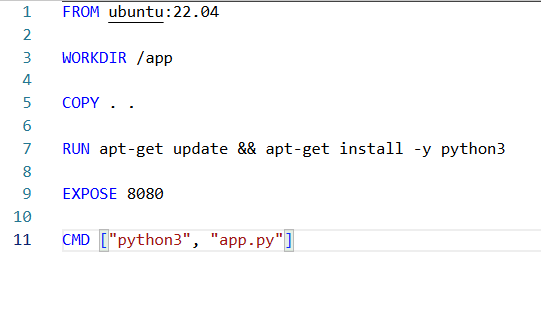
\includegraphics[width=0.75\textwidth]{pics/dockerfile.png}
    \caption{Beispiel eines einfachen Dockerfiles}
    \label{fig:dockerfile-example}
\end{figure}

\texttt{FROM} gibt an welches Basis-Image verwendet wird, also 
quasi das Betriebssystem auf dem die Anwendung läuft, zum 
Beispiel \texttt{FROM ubuntu:22.04}.

\texttt{WORKDIR} legt fest in welchem Ordner innerhalb des 
Containers gearbeitet wird, ähnlich wie ein \texttt{cd} Befehl 
im Terminal.

\texttt{COPY} kopiert Dateien vom eigenen Rechner in das Image, 
zum Beispiel den Quellcode der Anwendung.

\texttt{RUN} führt einen Befehl aus während das Image gebaut 
wird, zum Beispiel das Installieren von Abhängigkeiten mit 
\texttt{npm install}.

\texttt{EXPOSE} gibt an auf welchem Port die Anwendung 
erreichbar ist, zum Beispiel Port 8080 für ein Backend.

\texttt{CMD} definiert was passiert wenn der Container 
gestartet wird, also welcher Befehl die Anwendung startet.

\subsubsection{Multi-Stage Builds}

Ein wichtiges Konzept sind \textbf{Multi-Stage Builds}. Dabei wird 
das Dockerfile in mehrere Phasen unterteilt, wobei jede Phase ein 
eigenes Basis-Image verwenden kann \cite{docker_dockerfile}.

Der Vorteil ist, dass Build-Werkzeuge wie Compiler oder Paketmanager 
nur in der Build-Phase benötigt werden und nicht im finalen Image 
landen. Das Ergebnis ist ein deutlich schlankeres und sichereres 
Produktiv-Image, da unnötige Tools keine potenzielle Angriffsfläche 
bieten \cite{docker_dockerfile}.

\begin{figure}[H]
    \centering
    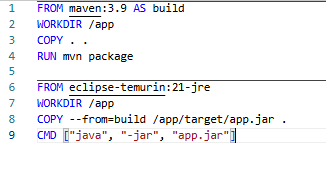
\includegraphics[width=0.75\textwidth]{pics/multistage_example.png}
    \caption{Prinzip eines Multi-Stage Builds}
    \label{fig:multistage-example}
\end{figure}